\section{Heurística de búsqueda local}
\subsection{Descripción de los algoritmos}
El procedimiento de una heurística de busqueda local consiste en tomar una solución inicial $s$ cualquiera e iterativamente mejorarla remplazandola por una solución mejor del conjunto de soluciones vecinas ($N(s)$ definidas particularmente en cada algoritmo), hasta llegar a un óptimo local.

Llamamos heurística de busqueda local al método de selección que usamos para elegir o descartar una vecindad. Los algoritmos implementados a continuación usan el mismo criterio de heurística que consiste en iterar sobre las vecindades y elegir la primera que mejora la solución. Usamos este criterio por que mejora el tiempo de ejecución ya que cuando encuentra una mejor la elige y por que no encontramos otra considerablemente mejor. Por ejemplo se podría haber propuesto una heurística que recorra todas las vecindades y elija la mejor opción entre todas, pero aun en el mejor caso deberiamos recorrer todas las soluciones de $N(s)$ y esto incrementa el costo temporal.

Implementamos dos tipos de vecindades: \textbf{(A)} toma un nodo de alguno de los $k$ subconjuntos y prueba si cambiando este nodo de subconjunto mejora el valor de la solución, siendo la vecindad todas las soluciones que difieren de la actual con un solo nodo en otro subconjunto $k$. \textbf{(B)} consiste en intercambiar dos nodos cualesquiera de distintos subconjuntos y ver si el valor mejora, es decir que la vecindad son aquellas soluciones que difieren solamente con un intercambio de nodos en dos distintos subconjuntos.

Consideramos que la implementación que tiene la vecindad de tipo \textbf{(B)} es más limitada que la \textbf{(A)} porque la \textbf{(B)} mantiene la cardinalidad en los subconjuntos de la solución (ya que solo hace swap entre nodos de distintos subconjuntos) y esto hace que el algoritmo este más condicionado por la solución de partida.

\textbf{(A)}:
\begin{algorithm}[H]
\begin{algorithmic}[1]
\caption{HeuristicaBusquedaLocal(Grafo G, nat k)}
\STATE Vector$<$Conjunto$<$Nat$>>$ conjuntos(k, vacío)
\STATE solucionInicial(G,k)
\STATE Bool hayMejora $\leftarrow$ true
\WHILE {hayMejora}
    \STATE hayMejora $\leftarrow$ false
    \FOR {\textbf{each} nodos}
        \STATE Bool swappeado $\leftarrow$ false
        \STATE Int subset $\leftarrow$ 0
        \WHILE {!swappeado y subset $<$ k}
            \IF{subset != subcjtoDel(nodo) y pesoDelNodoEnSubcjto(actual) $>$ pesoDelNodoEnSubcjto(subset)}
                \STATE borroNodoDeSubcjto(nodo,actual)
                \STATE agregoNodoASubcjto(nodo,subset)
                \STATE hayMejora $\leftarrow$ true
                \STATE swappeado $\leftarrow$ true
            \ENDIF
            \STATE subset++
        \ENDWHILE
    \ENDFOR
\ENDWHILE
\RETURN conjuntos
\end{algorithmic}
\end{algorithm}

\textbf{(B)}:
\begin{algorithm}[H]
\begin{algorithmic}[1]
\caption{HeuristicaBusquedaLocalConSwap(Grafo G, nat k)}
\STATE Vector$<$Conjunto$<$Nat$>>$ conjuntos(k, vacío)
\STATE solucionInicial(G,k)
\STATE Bool hayMejora $\leftarrow$ true
\WHILE {hayMejora}
    \STATE hayMejora $\leftarrow$ false
    \FOR {\textbf{each} nodos}
        \STATE Bool swappeado $\leftarrow$ false
        \STATE nodoSwap $\leftarrow$ nodo$+1$
        \WHILE {!swappeado y nodoSwap $<$ n}
            \IF{subcjtoDel(nodo) != subcjtoDel(nodoSwap)}
                \STATE pesoNodoCambiado $\leftarrow$ pesoDelNodoEnSubcjto(nodo,subcjtoDel(nodoSwap))
                \STATE pesoNodoSwapCambiado $\leftarrow$ pesoDelNodoEnSubcjto(nodoSwap,subcjtoDel(nodo))
                \IF{peso(nodo)$+$peso(nodoSwap) $>$ pesoNodoCambiado$+$pesoNodoSwapCambiado}
                    \STATE borroNodoDeSubcjto(nodo,subcjtoDel(nodo))
                    \STATE agregoNodoASubcjto(nodo,subcjtoDel(nodoSwap))
                    \STATE borroNodoDeSubcjto(nodoSwap,subcjtoDel(nodoSwap))
                    \STATE agregoNodoASubcjto(nodoSwap,subcjtoDel(nodo))
                    \STATE hayMejora $\leftarrow$ true
                    \STATE swappeado $\leftarrow$ true
                \ENDIF
            \ENDIF
            \STATE nodoSwap++
        \ENDWHILE
    \ENDFOR
\ENDWHILE
\RETURN conjuntos
\end{algorithmic}
\end{algorithm}

Ejemplo de ejecución de los algoritmos:

Tenemos el siguiente grafo de entrada, y nos piden correr los algoritmos para $k=3$

\begin{figure}[H]
    \centering
    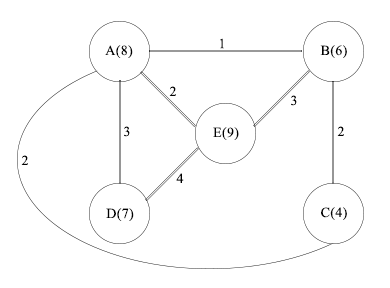
\includegraphics[scale=0.7]{ejercicio-4-ejemplo-entrada.png}
    \caption{Grafo de entrada}
    \label{fig:ej4_ejemplo}
\end{figure}

Contamos con la siguiente solución inicial (entre parentesis el peso de cada nodo):
\begin{center}
  \begin{tabular}{ l | c | r }
    $S_{1}$ & $S_{2}$ & $S_{3}$ \\ \hline
    A(3) & E(0) & D(0) \\
    B(4) &  &  \\
    C(3) &  &  \\
  \end{tabular}
  \textbf{Costo total:} 5
\end{center}

\begin{minipage}[t]{0.5\linewidth}
    \center{\textbf{(A)}} \\
    \raggedright{
        \textit{Tomo A:}\\
        $\rightarrow$ Lo pruebo en $S_{2}$: A(2) \checkmark Mejora
    }\\
    \begin{center}
      \begin{tabular}{ l | c | r }
        $S_{1}$ & $S_{2}$ & $S_{3}$ \\ \hline
        B(2) & E(2) & D(0) \\
        C(2) & A(2) &  \\
      \end{tabular}
      \textbf{Costo total:} 4
    \end{center}

    \raggedright{
        \textit{Tomo B:}\\
        $\rightarrow$ Lo pruebo en $S_{2}$: B(4) No mejora\\
        $\rightarrow$ Lo pruebo en $S_{3}$: B(0) \checkmark Mejora
    }\\
    \begin{center}
      \begin{tabular}{ l | c | r }
        $S_{1}$ & $S_{2}$ & $S_{3}$ \\ \hline
        C(0) & E(2) & D(0) \\
         & A(2) & B(0) \\
      \end{tabular}
      \textbf{Costo total:} 2
    \end{center}

    \raggedright{
        \textit{Tomo C:}\\
        $\rightarrow$ Lo pruebo en todos pero no mejora en ninguno por que tiene peso 0.
    }\\

    \raggedright{
        \textit{Tomo D:}\\
        $\rightarrow$ Lo pruebo en todos pero no mejora en ninguno por que tiene peso 0.
    }\\

    \raggedright{
        \textit{Tomo E:}\\
        $\rightarrow$ Lo pruebo en $S_{1}$: E(0) \checkmark Mejora
    }\\
    \begin{center}
      \begin{tabular}{ l | c | r }
        $S_{1}$ & $S_{2}$ & $S_{3}$ \\ \hline
        C(0) & A(0) & D(0) \\
        E(0) &  & B(0) \\
      \end{tabular}
      \textbf{Costo total:} 0
    \end{center}

    Hace una iteración mas buscando mejora pero no la encuentra, entonces termina. 

\end{minipage}
\vrule
\begin{minipage}[t]{0.5\linewidth}
    \centering{\textbf{(B)}}\\
    \raggedright{
        \textit{Tomo A y B:}\\
        $\rightarrow$ estan en el mismo subconjunto (no hago nada).
    }\\
    \raggedright{
        \textit{Tomo A y C:}\\
        $\rightarrow$ estan en el mismo subconjunto.
    }\\
    \raggedright{
        \textit{Tomo A y D:}\\
        $\rightarrow$ como peso(A en $S_{3}$ sin D)$+$peso(D en $S_{1}$ sin A) $<$ peso(A actual)+peso(D actual)
    }\\
    \begin{center}
      \begin{tabular}{ l | c | r }
        $S_{1}$ & $S_{2}$ & $S_{3}$ \\ \hline
        B(2) & E(0) & A(0) \\
        C(2) &  &  \\
        D(0) &  &  \\
      \end{tabular}
      \textbf{Costo total:} 2
    \end{center}
    \raggedright{
        \textit{Tomo B y A:}\\
        $\rightarrow$ no mejora.
    }\\
    \raggedright{
        \textit{Tomo B y C:}\\
        $\rightarrow$ estan en el mismo subconjunto.
    }\\
    \raggedright{
        \textit{Tomo B y D:}\\
        $\rightarrow$ estan en el mismo subconjunto.
    }\\
    \raggedright{
        \textit{Tomo B y E:}\\
        $\rightarrow$ no mejora.
    }\\
    \raggedright{
        \textit{Tomo C y A:}\\
        $\rightarrow$ no mejora.
    }\\
    \raggedright{
        \textit{Tomo C y B:}\\
        $\rightarrow$ estan en el mismo subconjunto.
    }\\
    \raggedright{
        \textit{Tomo C y D:}\\
        $\rightarrow$ estan en el mismo subconjunto.
    }\\
    \centering{...}\\
    No mejora en ninguna de las combinaciones siguientes.
    Termina.


\end{minipage}


\subsection{Análisis de complejidad temporal}
Sea $n$ la cantidad de vértices del grafo de entrada, y $k$ el parámetro de k-PMP. Vamos a usar el pseudocódigo ya introducido para el cálculo de complejidad de ambos algoritmos. Hay que mencionar que ésta se calcula para el peor caso de una iteración del ciclo más exterior de los algoritmos (\textit{while(hayMejora)}) ya que no podemos determinar cuantas veces se itera sobre este mismo. Lo que si se afirma es que termina cuando encuentra un óptimo local, es decir ninguno de sus vecinos tiene una mejor solución. Se omite la complejidad de la obtención de la solución inicial y se asume como entrada.
\\

\textbf{(A):}

\begin{itemize}
    \item Linea $5$: seteamos la variable \textit{hayMejora} en $O(1)$
    \item Linea $6$: iniciamos un ciclo que se repite n veces.
    \begin{itemize}
        \item Lineas $7$ y $8$: seteamos variables en $O(1)$ y calculamos el peso del nodo en cuestión en el subconjunto esto cuesta $O(n)$ (si bien no está explícito en el pseudocódigo, realizamos este preproceso para no realizarlo dentro del ciclo siguiente y así aumentar su complejidad innecesariamente.)
        \item Linea $9$: Se inicia otro ciclo sobre los subconjuntos que como peor caso se prueba cambiar el nodo a todos los subconjuntos y recorremos los $k$.
        \begin{itemize}
            \item Linea $10$: Checkeo booleano del if en $O(1)$
            \item Lineas $11$, $12$, $13$ y $14$: borrar e insertar nodos de un conjunto cuesta $O(\log n)$ y las asignaciones de variables $O(1)$. 

            Entonces tenemos $2O(\log n) + 2O(1)$

            Cómo peor caso esto ocurre una vez en las $k$ iteraciones ya que hace que salgamos de él.
            \item Linea $16$: aumentamos una variable en $O(1)$
        \end{itemize}
    \end{itemize}
\end{itemize}
Entonces tenemos:
\begin{center}
    $Complejidad(A) = O(1) + n(O(1)+O(n)+O(k)+2O(\log n)+2O(1)+O(1))$

    $Complejidad(A) = n(max\{O(n),O(k),O(\log n)\})$

    $Complejidad(A) = max\{O(n^2),O(nk),O(n\log n)\}$

    $Complejidad(A) = O(n^2)$
\end{center}

\textbf{(B):}

\begin{itemize}
    \item Linea $5$: seteamos la variable \textit{hayMejora} en $O(1)$
    \item Linea $6$: iniciamos un ciclo que se repite n veces.
    \begin{itemize}
        \item Lineas $7$ y $8$: seteamos variables en $O(1)$ y calculamos los pesos de ambos nodos en los dos subconjuntos, esto cuesta $4O(n)$ (esto lo hacemos para no calcularlos dentro del siguiente ciclo.)
        \item Linea $9$: Se inicia otro ciclo sobre los nodos (para checkear con quien swappeo) en peor caso se repita $n$ veces.
        \begin{itemize}
            \item Linea $10$: Checkea booleano del if en $O(1)$
            \item Lineas $11$ y $12$: Calcula el valor del peso del nodo en un subconjunto, como peor caso esto toma $O(n)$
            \item Linea $13$: Checkea booleano del if en $O(1)$
            \item Lineas $14$ a $19$: Borra e inserta nodos de un subconjunto a otro, cuesta $O(\log n)$ y las asignaciones de variables $O(1)$. 

            Entonces tenemos $4O(\log n) + 2O(1)$

            Cómo peor caso esto ocurre una vez en las $n$ iteraciones ya que hace que salgamos de él.
            \item Linea $16$: aumentamos una variable en $O(1)$
        \end{itemize}
    \end{itemize}
\end{itemize}

Entonces tenemos:
\begin{center}
  $Complejidad(B) = O(1) + n(O(1)+4O(n)+n(O(n)+4O(\log n)+2O(1))+O(1))$

  $Complejidad(B) = n(O(n)+O(n^2))$ 

  $Complejidad(B) = O(n^3)$
\end{center}

\subsection{Experimentación de calidad}
Con esta experimentación nos interesan ver dos cosas:

\begin{enumerate}
  \item cuál de las dos vecindades obtiene soluciones de mejor calidad.
  \item cuál de las dos vecindades \textit{gana} más veces que la otra. 
    Por ganar nos referimos a que obtiene una partición de menor peso.
\end{enumerate}

Para evaluarlo generamos un set de instancias que se compone de 100 instancias por $n$, siendo
$n$ la cantidad de nodos de la instancia, con $3 \leq n \leq 22$. La limitante para aumentar más
el $n$ es que el tiempo del exacto, incluso con todas las podas, crece demasiado rápido y para
poder saber cuán lejos estaban los pesos obtenidos por las heurísticas de búsqueda local era necesario
correr el algoritmo exacto. En todas las instancias las búsquedas para las dos vecindades parten de
la misma partición inicial que es la generada por el goloso sin aleatorización. Creemos que 
empezar desde la solución obtenida por la golosa se acerca un más al uso real que va a tener en 
comparación con empezar con una partición completamente aleatoria, por lo cual los resultados que
obtengamos serán más representativos del comportamiento que vayan a tener en su contexto de uso.
Los valores graficados se corresponden con los promedios de pesos por instancia. Es necesario
aclarar que limitamos el número de iteraciones de las dos búsquedas locales a 100. Creemos
que esto es importante ya que no sólo nos interesa controlar que la calidad de las soluciones que 
estamos comparando hayan sido obtenidas dentro de el mismo número de iteraciones. De no haber hecho esto
una de las dos podría haber superado a la otra pero realizando muchas más iteraciones. Sumamos los pesos
obtenidos para las 100 instancias de cada $n$ y luego tomamos el promedio. El promedio no es un buen 
indicador en muchos casos ya que no nos habla en general de la dispersión de los resultados. Para
darnos una idea de cuán estable son los resultados que obtienen cada una de las vecindades necesitaríamos
obtener también el desvío estándar. Sin embargo, los promedios de las dos vecindades han quedado con error
relativo pequeño con respecto al peso obtenido por el algoritmo exacto por lo cual el desvío estándar debe ser pequeño
ya que no pueden haber valores por debajo del exacto para compensar otros muy altos.

\begin{figure}[H]
		\centering
		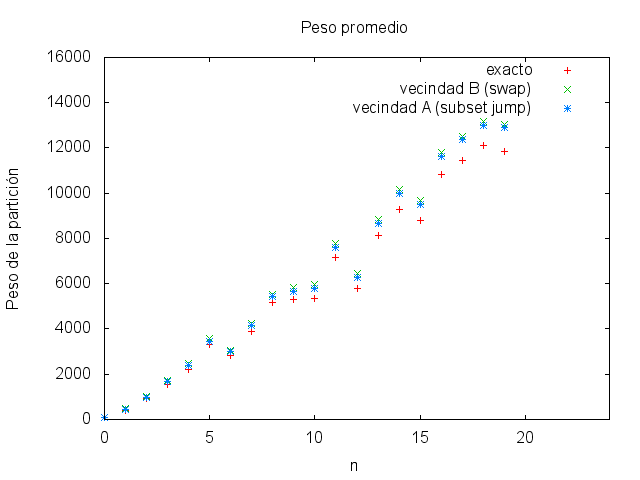
\includegraphics[width=\textwidth]{calidad_trendline.png}
		\caption{Pesos promedio.}
		\label{fig:ej3_ejemplo}
\end{figure}

La distancia entre los pesos obtenidos por las vecindades y el exacto se mantiene parece estar creciendo.
No obstante, la distancia entre las dos vecindades se mantiene, a simple vista, constante. La vecindad A, que
corresponde a la que cambia de subconjunto a un nodo, siempre se ubica por debajo de la vecindad B, correspondiente
a la de swap, pero por un margen muy pequeño. Sobre todo para las instancias donde el $n$ es más grande, superior
a 15, los resultados dejan de seguir una curva suave lo cual interpretamos que se debe a que 100 instancias a medida
que el $n$ aumenta deja de ser un valor representativo.
Además, realizamos un histograma que muestra para cada $n$ qué vecindad obtuvo el menor peso de las dos para cada una
de las 100 instancias. De esta forma podemos ver más claramente cuál ganó más veces, otro indicador de cuál podría
llegar a ser superior.

\begin{figure}[H]
		\centering
		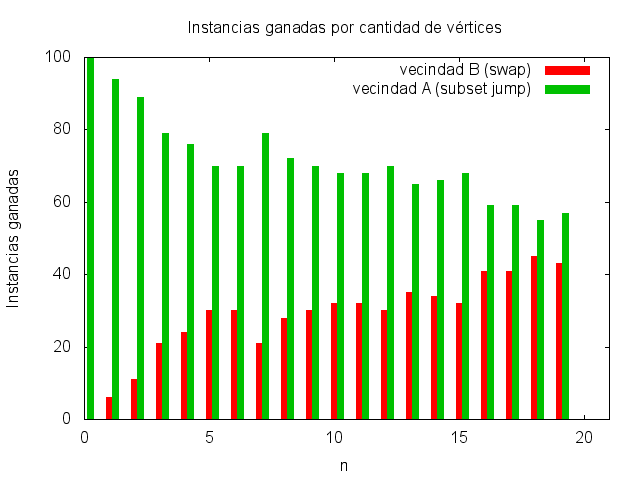
\includegraphics[width=\textwidth]{calidad_histograma.png}
		\caption{Instancias ganadas.}
		\label{fig:ej3_ejemplo}
\end{figure}

Vemos que la vecindad A comienza con una ampli ventaja sobre la vecindad B pero a medida que el $n$ aumenta
se va emparejando cada vez más. Ésta es una tendendia que no habíamos podido apreciar en el gráfico de pesos.
No estamos seguros si se debe a como ya mencionamos la falta de representatividad de las 100 instancias para
los $n$ más grandes o a que efectivamente la vecindad A obtiene soluciones de mejor calidad en la mayoría de los
casos.

\subsection{Experimentación de complejidad}
En esta experimentación simplemente queremos ganar confianza en las cotas de complejidad
calculadas teóricamente. Recordamos que para la vecindad A (cambio de subconjunto) la cota obtenida
había sido $O(n^2)$. Lo que hicimos fue correr el mismo conjunto de instancias que para la experimentación
de calidad pero aumentando el rango de valores de que toma $n$ ya que en este caso no es necesario correr
el algoritmo exacto que nos limitaba anteriormente. Los tiempos están divididos por $n$.

\begin{figure}[H]
		\centering
		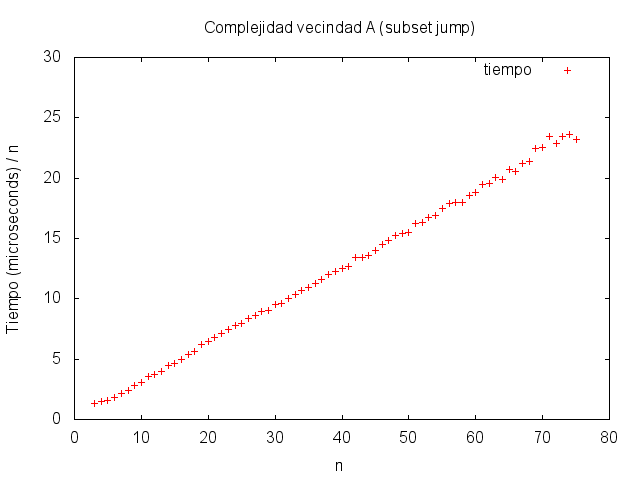
\includegraphics[width=\textwidth]{tiempos_vecindad_a.png}
		\caption{Instancias ganadas.}
		\label{fig:ej3_ejemplo}
\end{figure}

Los tiempos parecen presentar un comportamiento bastante definido incluso para valores de $n$ más grandes
por lo cual creemos que la cota de complejidad se acerca lo suficiente a la real.
Realizamos lo mismo para la vecindad B (swap). Recordamos que la cota obtenida para ésta vecindad era $O(n^3)$
por lo cual dividimos los tiempos por $n^2$.

\begin{figure}[H]
		\centering
		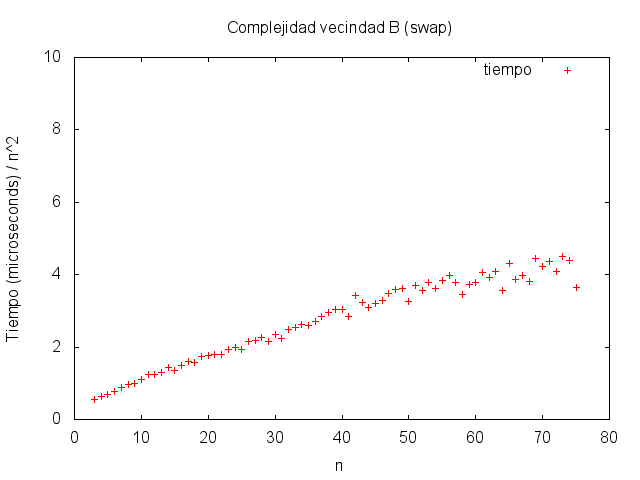
\includegraphics[width=\textwidth]{tiempos_vecindad_b.png}
		\caption{Instancias ganadas.}
		\label{fig:ej3_ejemplo}
\end{figure}

En este caso vemos que si bien parece que los valores exhiben un crecimiento lineal, a partir de $n = 40$
esta tendencia se vuelve cada vez más endeble ya que los valores empiezan a presentar turbulencia. Creemos
que una vez más esto puede deberse a la falta de representatividad de un valor de sólo 100 instancias para
un número de nodos tan grandes, lo cual podría resultar en instancias muy densas y otras muy simples.
Concluimos que la vecindad A por tener una complejidad menor y mostrarse levemente superior en cuanto
a calidad de las soluciones obtenidas con respecto a la vecindad B será una mejor elección para nuestra
implementación de la metaheurística GRASP.
